\documentclass{standalone}
\usepackage{tikz}
\usetikzlibrary{patterns, positioning}
\usepackage[sfdefault]{ClearSans} %% option 'sfdefault' activates Clear Sans as the default text font
\usepackage[T1]{fontenc}

\begin{document}
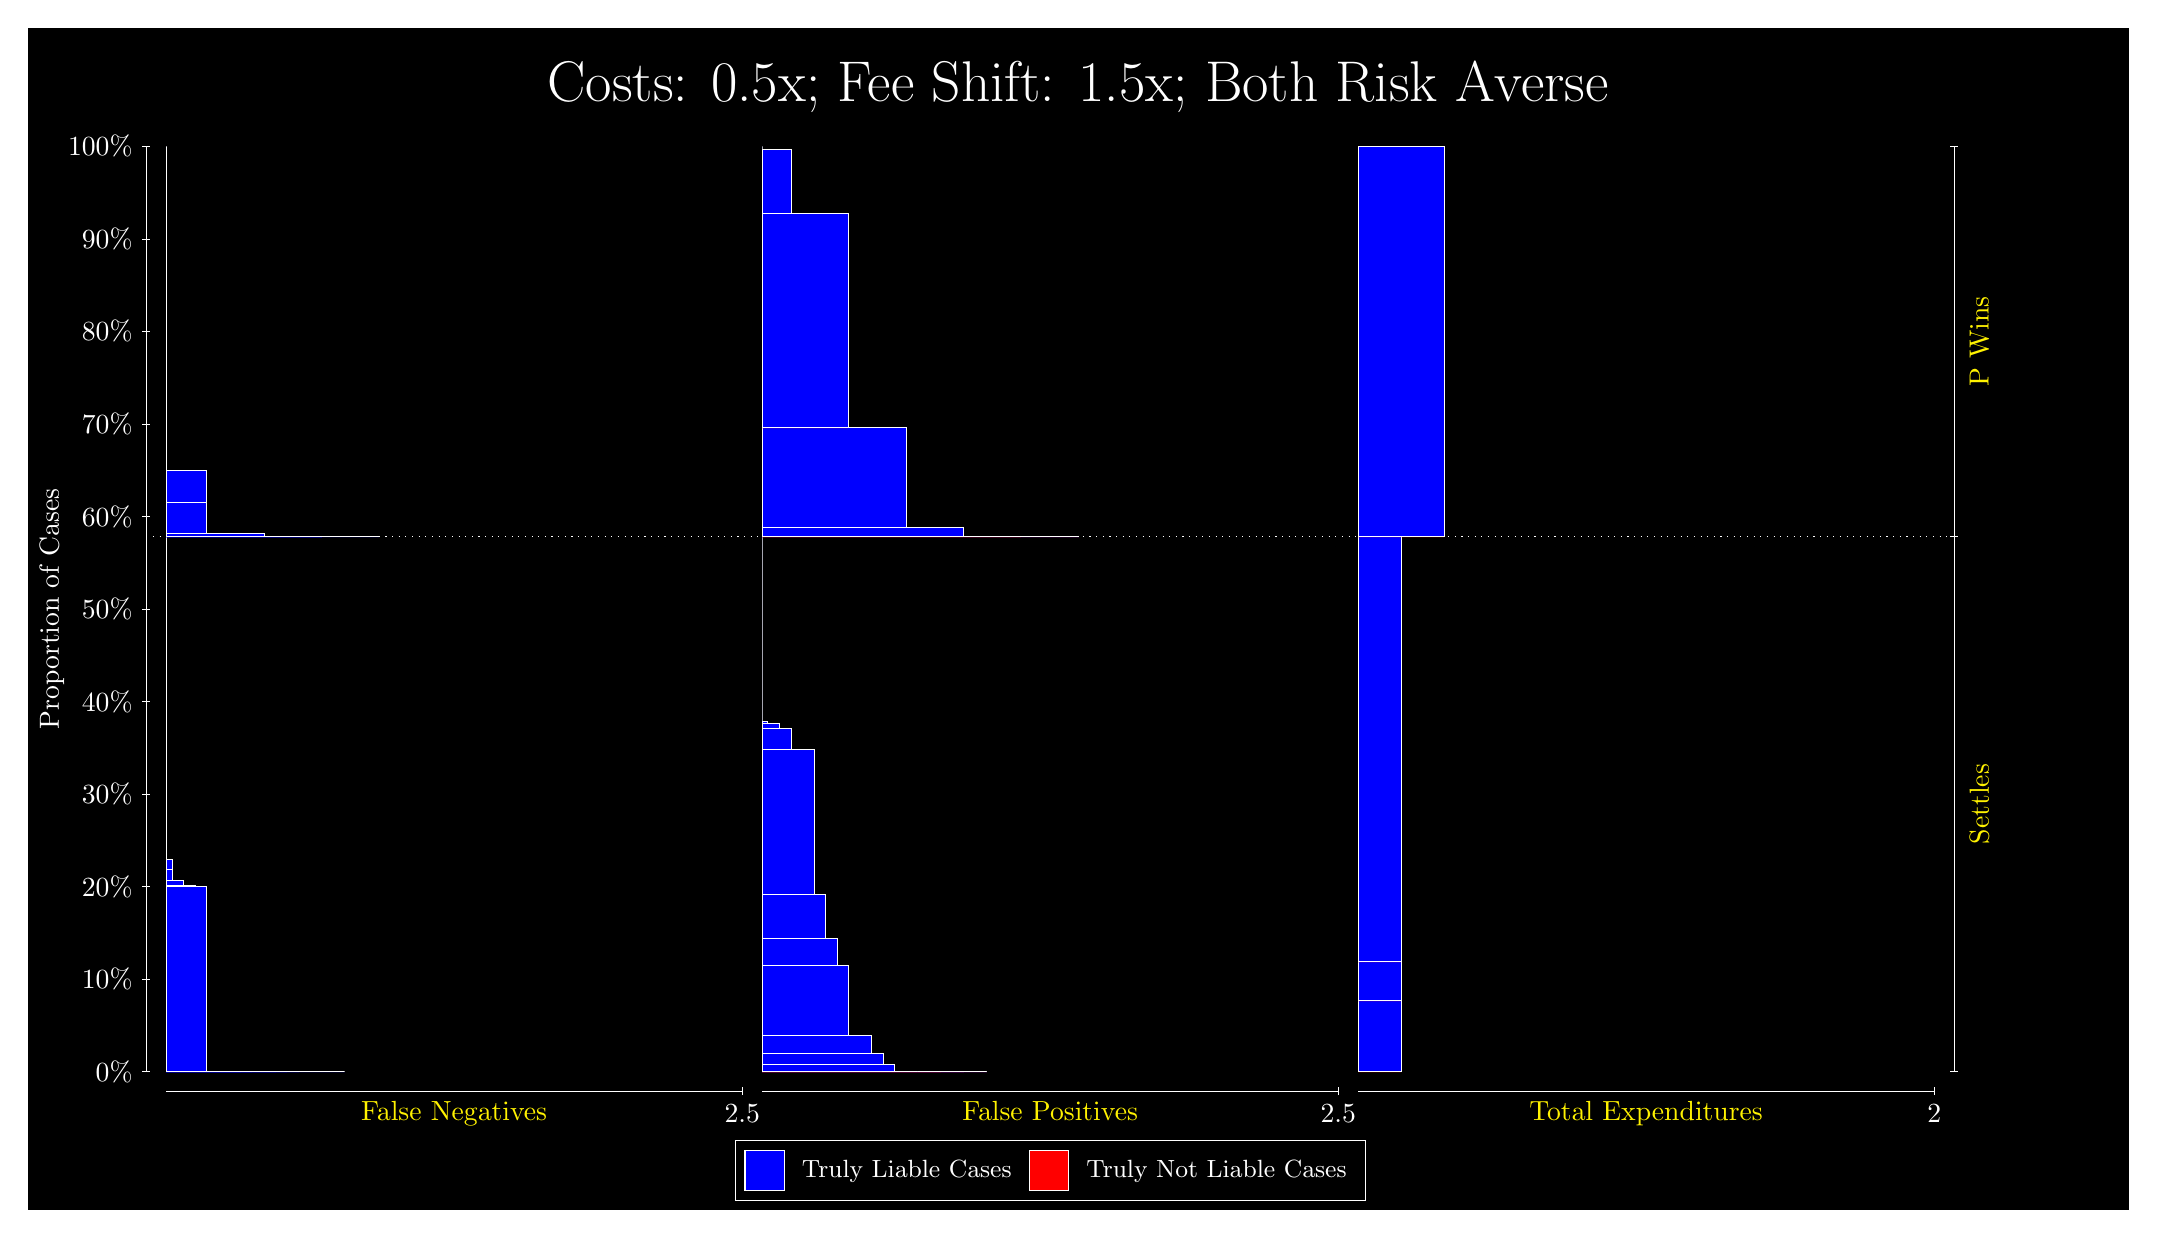
\begin{tikzpicture}
\draw[fill=black] (0,0) rectangle (26.667,15);
\draw[text=white] (0,13.5) rectangle (26.667,15) node[midway] {\huge Costs: 0.5x; Fee Shift: 1.5x; Both Risk Averse};
\draw[white, very thin] (1.5,1.75) -- (1.5,13.5);
\node[rotate=90, text=white, anchor=center] at (0.3, 7.625) {Proportion of Cases};
\draw[white, very thin] (1.45,1.75) -- (1.55,1.75);
\node[text=white, anchor=east] at (1.45, 1.75) {0\%};
\draw[white, very thin] (1.45,2.925) -- (1.55,2.925);
\node[text=white, anchor=east] at (1.45, 2.925) {10\%};
\draw[white, very thin] (1.45,4.1) -- (1.55,4.1);
\node[text=white, anchor=east] at (1.45, 4.1) {20\%};
\draw[white, very thin] (1.45,5.275) -- (1.55,5.275);
\node[text=white, anchor=east] at (1.45, 5.275) {30\%};
\draw[white, very thin] (1.45,6.45) -- (1.55,6.45);
\node[text=white, anchor=east] at (1.45, 6.45) {40\%};
\draw[white, very thin] (1.45,7.625) -- (1.55,7.625);
\node[text=white, anchor=east] at (1.45, 7.625) {50\%};
\draw[white, very thin] (1.45,8.8) -- (1.55,8.8);
\node[text=white, anchor=east] at (1.45, 8.8) {60\%};
\draw[white, very thin] (1.45,9.975) -- (1.55,9.975);
\node[text=white, anchor=east] at (1.45, 9.975) {70\%};
\draw[white, very thin] (1.45,11.15) -- (1.55,11.15);
\node[text=white, anchor=east] at (1.45, 11.15) {80\%};
\draw[white, very thin] (1.45,12.325) -- (1.55,12.325);
\node[text=white, anchor=east] at (1.45, 12.325) {90\%};
\draw[white, very thin] (1.45,13.5) -- (1.55,13.5);
\node[text=white, anchor=east] at (1.45, 13.5) {100\%};

\draw[white, very thin] (24.457,1.75) -- (24.457,13.5);
\draw[white, very thin] (24.407,1.75) -- (24.507,1.75);
\node[anchor=west] at (24.407, 1.75) {};
\draw[white, very thin] (24.407,8.5444) -- (24.507,8.5444);
\node[anchor=west] at (24.407, 8.5444) {};
\draw[white, very thin] (24.407,13.5) -- (24.507,13.5);
\node[anchor=west] at (24.407, 13.5) {};

\draw[white, very thin, fill=blue] (1.75,1.75) rectangle (4.0188,1.75);
\draw[white, very thin, fill=blue] (1.75,1.75) rectangle (3.4333,1.75);
\draw[white, very thin, fill=blue] (1.75,1.75) rectangle (3.287,1.75);
\draw[white, very thin, fill=blue] (1.75,1.75) rectangle (3.1406,1.75);
\draw[white, very thin, fill=blue] (1.75,1.75) rectangle (2.8478,1.75);
\draw[white, very thin, fill=blue] (1.75,1.75) rectangle (2.7015,1.7501);
\draw[white, very thin, fill=blue] (1.75,1.7501) rectangle (2.5551,1.7507);
\draw[white, very thin, fill=blue] (1.75,1.7507) rectangle (2.5551,1.7522);
\draw[white, very thin, fill=blue] (1.75,1.7522) rectangle (2.4087,1.7522);
\draw[white, very thin, fill=blue] (1.75,1.7522) rectangle (2.2623,4.0969);
\draw[white, very thin, fill=blue] (1.75,4.0969) rectangle (2.1159,4.121);
\draw[white, very thin, fill=blue] (1.75,4.121) rectangle (1.9696,4.184);
\draw[white, very thin, fill=blue] (1.75,4.184) rectangle (1.8232,4.3202);
\draw[white, very thin, fill=blue] (1.75,4.3202) rectangle (1.8232,4.4458);
\draw[white, very thin, fill=red] (1.75,4.4458) rectangle (1.75,4.4458);
\draw[white, very thin, fill=blue] (1.75,4.4458) rectangle (1.75,8.5444);
\draw[white, very thin, fill=blue] (1.75,8.5444) rectangle (4.458,8.5444);
\draw[white, very thin, fill=blue] (1.75,8.5444) rectangle (3.7261,8.5446);
\draw[white, very thin, fill=blue] (1.75,8.5446) rectangle (2.9942,8.5834);
\draw[white, very thin, fill=blue] (1.75,8.5834) rectangle (2.2623,8.9827);
\draw[white, very thin, fill=blue] (1.75,8.9827) rectangle (2.2623,9.3894);
\draw[white, very thin, fill=red] (1.75,9.3894) rectangle (1.75,9.3894);
\draw[white, very thin, fill=blue] (1.75,9.3894) rectangle (1.75,13.5);
\draw[white, very thin, fill=red] (9.3189,1.75) rectangle (12.173,1.75);
\draw[white, very thin, fill=blue] (9.3189,1.75) rectangle (12.173,1.75);
\draw[white, very thin, fill=red] (9.3189,1.75) rectangle (11.88,1.75);
\draw[white, very thin, fill=blue] (9.3189,1.75) rectangle (11.88,1.75);
\draw[white, very thin, fill=red] (9.3189,1.75) rectangle (11.588,1.75);
\draw[white, very thin, fill=blue] (9.3189,1.75) rectangle (11.588,1.7509);
\draw[white, very thin, fill=blue] (9.3189,1.7509) rectangle (11.441,1.7522);
\draw[white, very thin, fill=red] (9.3189,1.7522) rectangle (11.295,1.7522);
\draw[white, very thin, fill=blue] (9.3189,1.7522) rectangle (11.295,1.7522);
\draw[white, very thin, fill=blue] (9.3189,1.7522) rectangle (11.149,1.7533);
\draw[white, very thin, fill=red] (9.3189,1.7533) rectangle (11.002,1.7533);
\draw[white, very thin, fill=blue] (9.3189,1.7533) rectangle (11.002,1.8424);
\draw[white, very thin, fill=blue] (9.3189,1.8424) rectangle (10.856,1.9792);
\draw[white, very thin, fill=blue] (9.3189,1.9792) rectangle (10.709,2.2146);
\draw[white, very thin, fill=blue] (9.3189,2.2146) rectangle (10.563,2.2148);
\draw[white, very thin, fill=red] (9.3189,2.2148) rectangle (10.417,2.2148);
\draw[white, very thin, fill=blue] (9.3189,2.2148) rectangle (10.417,3.1023);
\draw[white, very thin, fill=blue] (9.3189,3.1023) rectangle (10.27,3.4465);
\draw[white, very thin, fill=blue] (9.3189,3.4465) rectangle (10.124,3.9978);
\draw[white, very thin, fill=blue] (9.3189,3.9978) rectangle (9.9776,5.8484);
\draw[white, very thin, fill=blue] (9.3189,5.8484) rectangle (9.8312,5.8486);
\draw[white, very thin, fill=blue] (9.3189,5.8486) rectangle (9.6848,6.1104);
\draw[white, very thin, fill=blue] (9.3189,6.1104) rectangle (9.5384,6.1735);
\draw[white, very thin, fill=blue] (9.3189,6.1735) rectangle (9.3921,6.1975);
\draw[white, very thin, fill=blue] (9.3189,6.1975) rectangle (9.3189,8.5444);
\draw[white, very thin, fill=red] (9.3189,8.5444) rectangle (13.344,8.5444);
\draw[white, very thin, fill=blue] (9.3189,8.5444) rectangle (13.344,8.5444);
\draw[white, very thin, fill=red] (9.3189,8.5444) rectangle (12.612,8.5444);
\draw[white, very thin, fill=blue] (9.3189,8.5444) rectangle (12.612,8.546);
\draw[white, very thin, fill=red] (9.3189,8.546) rectangle (11.88,8.546);
\draw[white, very thin, fill=blue] (9.3189,8.546) rectangle (11.88,8.661);
\draw[white, very thin, fill=red] (9.3189,8.661) rectangle (11.149,8.661);
\draw[white, very thin, fill=blue] (9.3189,8.661) rectangle (11.149,9.9263);
\draw[white, very thin, fill=red] (9.3189,9.9263) rectangle (10.417,9.9263);
\draw[white, very thin, fill=blue] (9.3189,9.9263) rectangle (10.417,12.655);
\draw[white, very thin, fill=blue] (9.3189,12.655) rectangle (9.6848,13.461);
\draw[white, very thin, fill=blue] (9.3189,13.461) rectangle (9.3189,13.5);
\draw[white, very thin, fill=red] (16.888,1.75) rectangle (17.437,1.75);
\draw[white, very thin, fill=blue] (16.888,1.75) rectangle (17.437,2.649);
\draw[white, very thin, fill=red] (16.888,2.649) rectangle (17.437,2.649);
\draw[white, very thin, fill=blue] (16.888,2.649) rectangle (17.437,3.1454);
\draw[white, very thin, fill=red] (16.888,3.1454) rectangle (17.437,3.1454);
\draw[white, very thin, fill=blue] (16.888,3.1454) rectangle (17.437,8.5444);
\draw[white, very thin, fill=red] (16.888,8.5444) rectangle (17.986,8.5444);
\draw[white, very thin, fill=blue] (16.888,8.5444) rectangle (17.986,13.5);
\draw[white, dotted] (1.5,8.5444) -- (24.457,8.5444);
\draw[white, very thin] (1.75,1.5) -- (9.0689,1.5);
\node[text=yellow, anchor=north] at (5.4094, 1.5) {False Negatives};
\draw[white, very thin] (9.0689,1.45) -- (9.0689,1.55);
\node[text=white, anchor=north] at (9.0689, 1.45) {2.5};

\draw[white, very thin] (9.3189,1.5) -- (16.638,1.5);
\node[text=yellow, anchor=north] at (12.978, 1.5) {False Positives};
\draw[white, very thin] (16.638,1.45) -- (16.638,1.55);
\node[text=white, anchor=north] at (16.638, 1.45) {2.5};

\draw[white, very thin] (16.888,1.5) -- (24.207,1.5);
\node[text=yellow, anchor=north] at (20.547, 1.5) {Total Expenditures};
\draw[white, very thin] (24.207,1.45) -- (24.207,1.55);
\node[text=white, anchor=north] at (24.207, 1.45) {2};

\node[text=yellow, centered, rotate=90] at (24.777, 5.1472) {Settles};
\node[text=yellow, centered, rotate=90] at (24.777, 11.022) {P Wins};

\draw (12.978300999999998,1.5) node[draw=none] (baseCoordinate) {};
\begin{scope}[align=center]
        \matrix[scale=0.5, draw=white, below=0.5cm of baseCoordinate, nodes={draw}, column sep=0.1cm]{
            \node[rectangle, draw, minimum width=0.5cm, minimum height=0.5cm, fill=blue] {}; &
            \node[draw=none, font=\small, text=white] (B) {Truly Liable Cases}; &
            \node[rectangle, draw, minimum width=0.5cm, minimum height=0.5cm, fill=red] {}; &
            \node[draw=none, font=\small, text=white] (B) {Truly Not Liable Cases}; \\
            };
\end{scope}

\end{tikzpicture}
\end{document}